\chapter{Implementation Details}
All source code is made available under \url{https;//github.com/fzimmermann89/msc}.
In \fref{algo:td} the procedure for time dependent simulations is show in detail.
\begin{algorithm}
	\caption{Time dependent Simulation}\label{timesim}
	\begin{algorithmic}
		\Procedure{Scan}{$x \in \mathbb{C}^N$, $t \in \mathbb{R}^N$, $\tau\ \in \mathbb{R}$}
		\Comment{Exponentially decaying inclusive prefix sum} 
		\State $s \gets 1$
		\While{$s<N$} 
		\Comment{Scan Upsweep}
		\For{k  $\gets 0$ to $N-1$ step $2s$ \textbf{parallel}}
		\State $decay \gets exp\left(\frac{t[k+s-1]-t[k+2s-1]}{\tau}\right)$ 
		\State $x[k+2s-1] \gets x[k+2s-1] + decay*x[k+s-1]$				
		\EndFor
		\State $s \gets 2s$ 
		\EndWhile
		\State $s \gets N/2$
		\While{$s>1$}  
		\Comment{Scan Downsweep}
		\State $s \gets s/2$
		\For{k  $\gets 0$ to $N-1-2s$ step $2s$ \textbf{parallel}}
		\State $decay \gets exp\left(\frac{t[k+2s-1]-t[k+3s-1]}{\tau}\right)$
		\State $x[k+3s-1] \gets x[k+3s-1] + decay*x[k+2s-1]$
		\EndFor
		\EndWhile
		\EndProcedure
		\Function {Prepare}{$x \in \mathbb{R}^{Nx3}$,  $y \in \mathbb{R}^{3}$, $t_0 \in \mathbb{R}^N$, $\phi \in [0,2\pi)^N$}
		\Comment{ommitted for brevity}
		\State \Return Time independent fields $a \in \mathbb{C}^N$, Arrival times $t \in \mathbb{R}^N$ for each atom
		\EndFunction
		\Function{Simulation}{Atom positions $x \in \mathbb{R}^{Nx3}$,  Detector position $y \in \mathbb{R}^{3}$, \newline Initial Phases $\phi \in [0,2\pi)^N$, Emission Times $t_0 \in \mathbb{R}^N$, $\tau\ \in \mathbb{R}$}
		\State	(a, t) = \Call {Prepare}{$x$, $y$, $\phi$}
		\State	\Call{Sort}{} ($a$,$t$) by $t$
		\State 	\Call{Scan}{$a$, $t$, $\tau$}
		\State $Result \gets \frac{\tau}{2} \left|a_N\right|^2 -\frac{\tau}{2}\sum_{n=1}^{N-1} \left|a_n\right|^2 \left(exp(-2 (t_{n+1}-t_n)/\tau)-1\right)$   
		\State \Return $Result$
		\EndFunction
		
	\end{algorithmic}
	\label{algo:td}
\end{algorithm}


The algorithm used to sample points a minimum distance apart from inside an n-dimensional volume used in the simulation of multiple samples inside the focal volume based on an algorithm first described by Bridson is shown in \fref{algo:bridson} \cite{bridson}. To draw random points uniformly from the annulus between $d$ and $2d$ around an existing point, the radius is sampled from the inverse of the radial CDF and the direction is generated using normalized n-dimensional normal distributed coordinates \cite{muller1959}.
An example of generated points is shown in \fref{fig:bridson}.
\begin{algorithm}
	\caption{Bridson's Poisson Sampling Algorithm}\label{algo:bridson}
	\begin{algorithmic}
		\Function{bridson}{ndim,d,r}
			\State $cellsize \gets d / \sqrt(ndim)$
			\State $grid \in \mathbb{Z}^{{{(2(r+d)/cellsize)}^{ndim}}} \gets 0$
			\State $Initialpoint \sim (2\mathcal{U}^2-1)*r$
			\State $queue \gets$ List(1)
			\State $points \gets$ List(Initialpoint)
			\While{queue}
				\State $ActivePoint \gets$ \textbf{pop} \textit{random element from queue}
				\Loop{k times}:
					\State $Candidate \gets$\Call{DrawCandidate}{$ActivePoint$}
					\If{\Call{Fits}{$Candidate$}}
						\State \textit{mark in grid}
						\State \textbf{add} $Candidate$ to $points$
						\State \textbf{add} $Candidate$ to $queue$
					\EndIf
				\EndLoop
			\EndWhile
			\State \Return $points$
		\EndFunction
		
		\Function {PointFits} {point, points, grid,d}:
			\State find points coordinate in grid
			\ForAll{cells less than d+cellsize away}
				\If{$cell\neq 0$}
					\State neighbor$\gets$ points[cell]
					 \If{$\left|neighbor-points\right|_2<d$} 	
					 	\State \Return False 
					 \EndIf
				\EndIf
			\EndFor
			\State \Return True
		\EndFunction
		\Function{DrawCandidate}{AroundPoint}
			\State $u \sim \mathcal{U}$
			\State $r \gets d * (1 + (2 ^ {ndim} - 1) * u) ^ {\sfrac{1}{ndim}}$
			\State $n \sim \mathcal{N}^{ndim}$
			\State \Return  $n/|n|_2 * r + AroundPoint$
		\EndFunction
	\end{algorithmic}
\end{algorithm}

\begin{figure}[H]
	\centering
	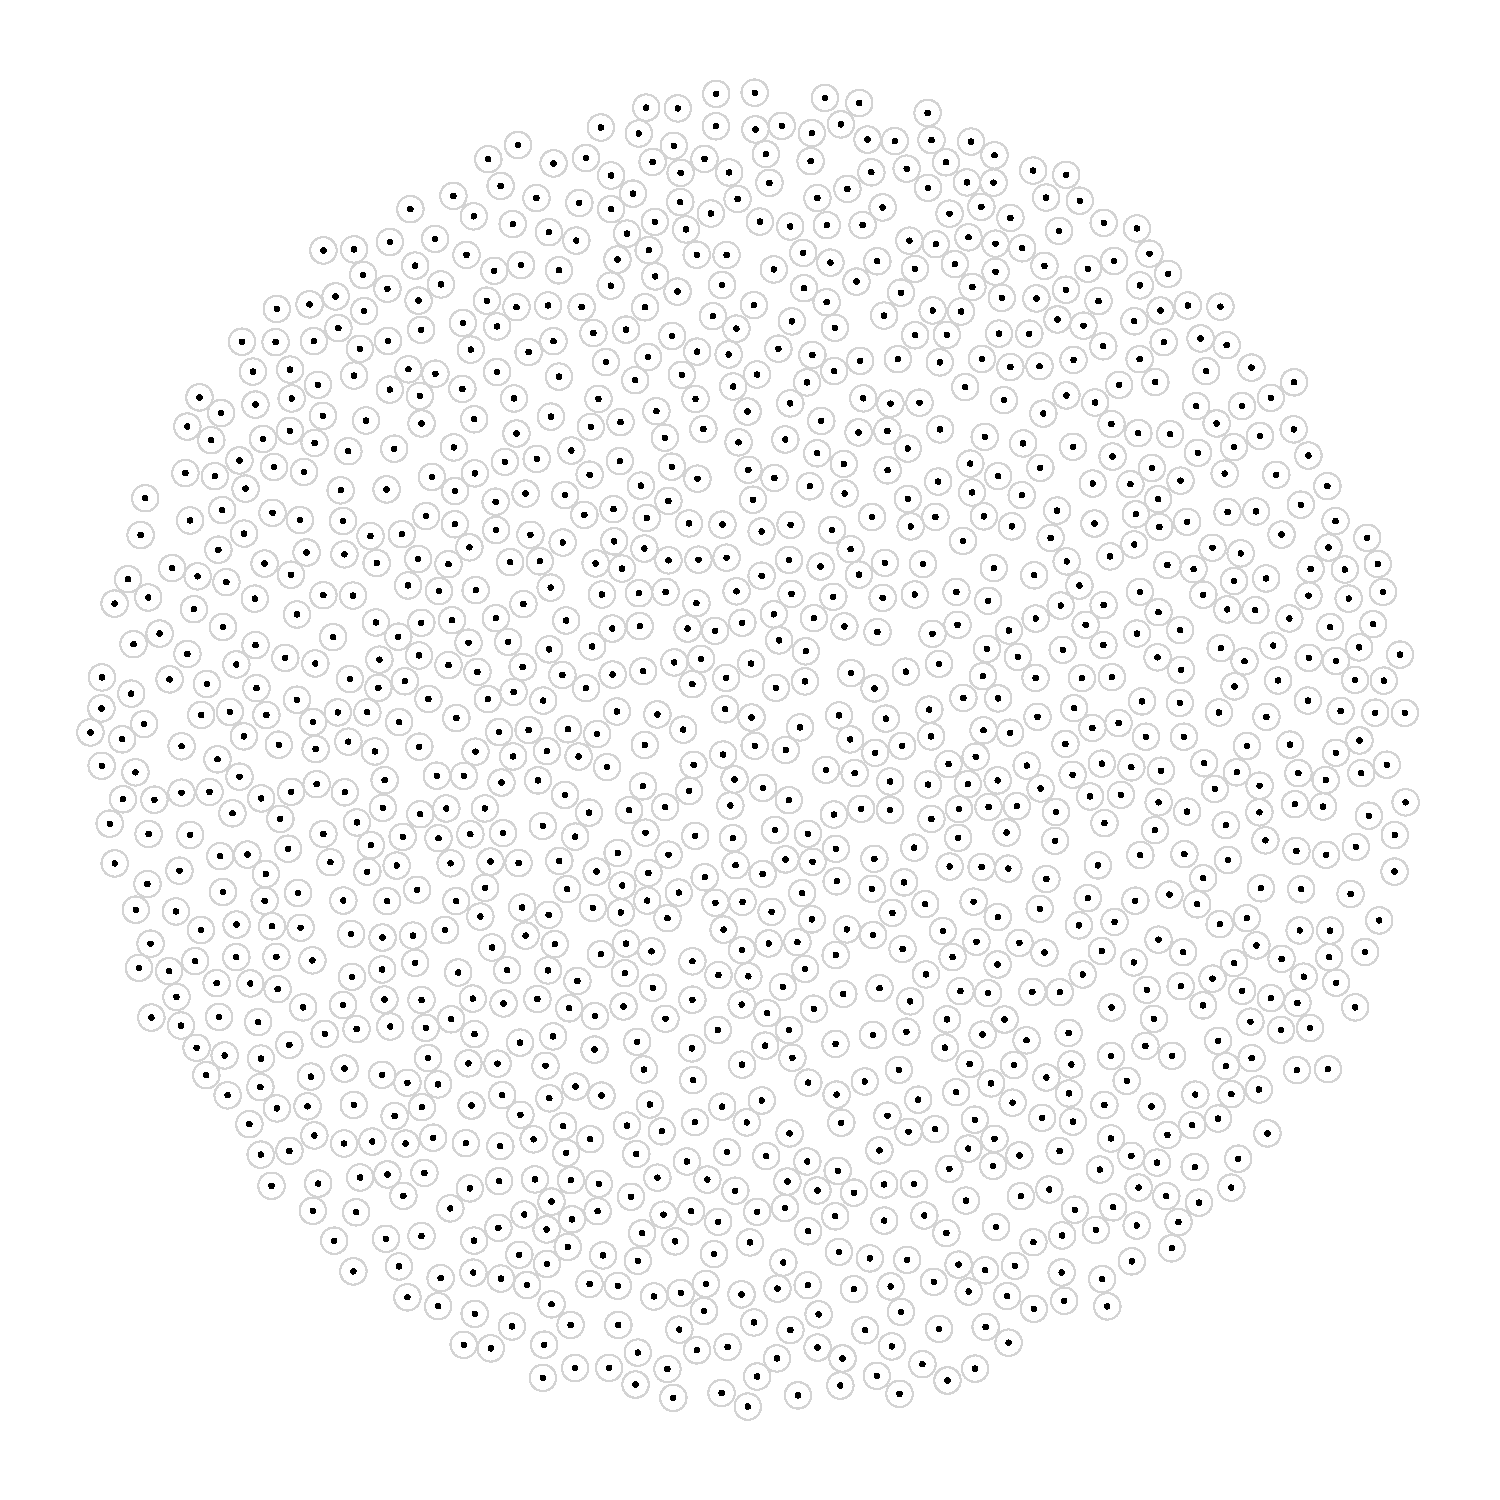
\includegraphics[width=0.4\linewidth]{images/bridson.pdf}
	\caption{Points generated by the Bridson algorithm inside a 2D circle (r=50) with a minimum distance of d=2.}
	\label{fig:bridson}
\end{figure}



\cite{born1980,griffiths2005}
\cite{mandel1995,baym1997,zernike1938,santra2009,sorum1987,lajunen04,tono2013}
